\documentclass[10pt,a4paper,sans]{moderncv}

% ModernCV themes
\moderncvstyle{classic}
\moderncvcolor{blue}

% Font configuration
\usepackage{fontspec}
\setmainfont{TeX Gyre Termes}
\setsansfont{TeX Gyre Heros}

% Icônes modernes
\usepackage{fontawesome5}

% Page margins
\usepackage[scale=0.85]{geometry}

% Hyperlinks
\usepackage[unicode,hidelinks]{hyperref}

% Personal data
\name{Camille}{Maslin}
\address{Tours, France}
\phone[mobile]{+33 6 25 87 56 93}
\email{camillemaslin@gmail.com}
\social[linkedin]{camille-maslin}
\social[github]{camille-maslin}
\extrainfo{\textbf{Portfolio :} \href{https://camille-maslin.github.io/Portfolio/}{\textcolor{blue}{camille-maslin.github.io/Portfolio}}}
\photo[80pt][0.4pt]{photo}

% En-tête moderne
\renewcommand*{\makecvtitle}{
  \vspace*{-1.5em}
  \parbox[b]{0.25\textwidth}{
    \centering
    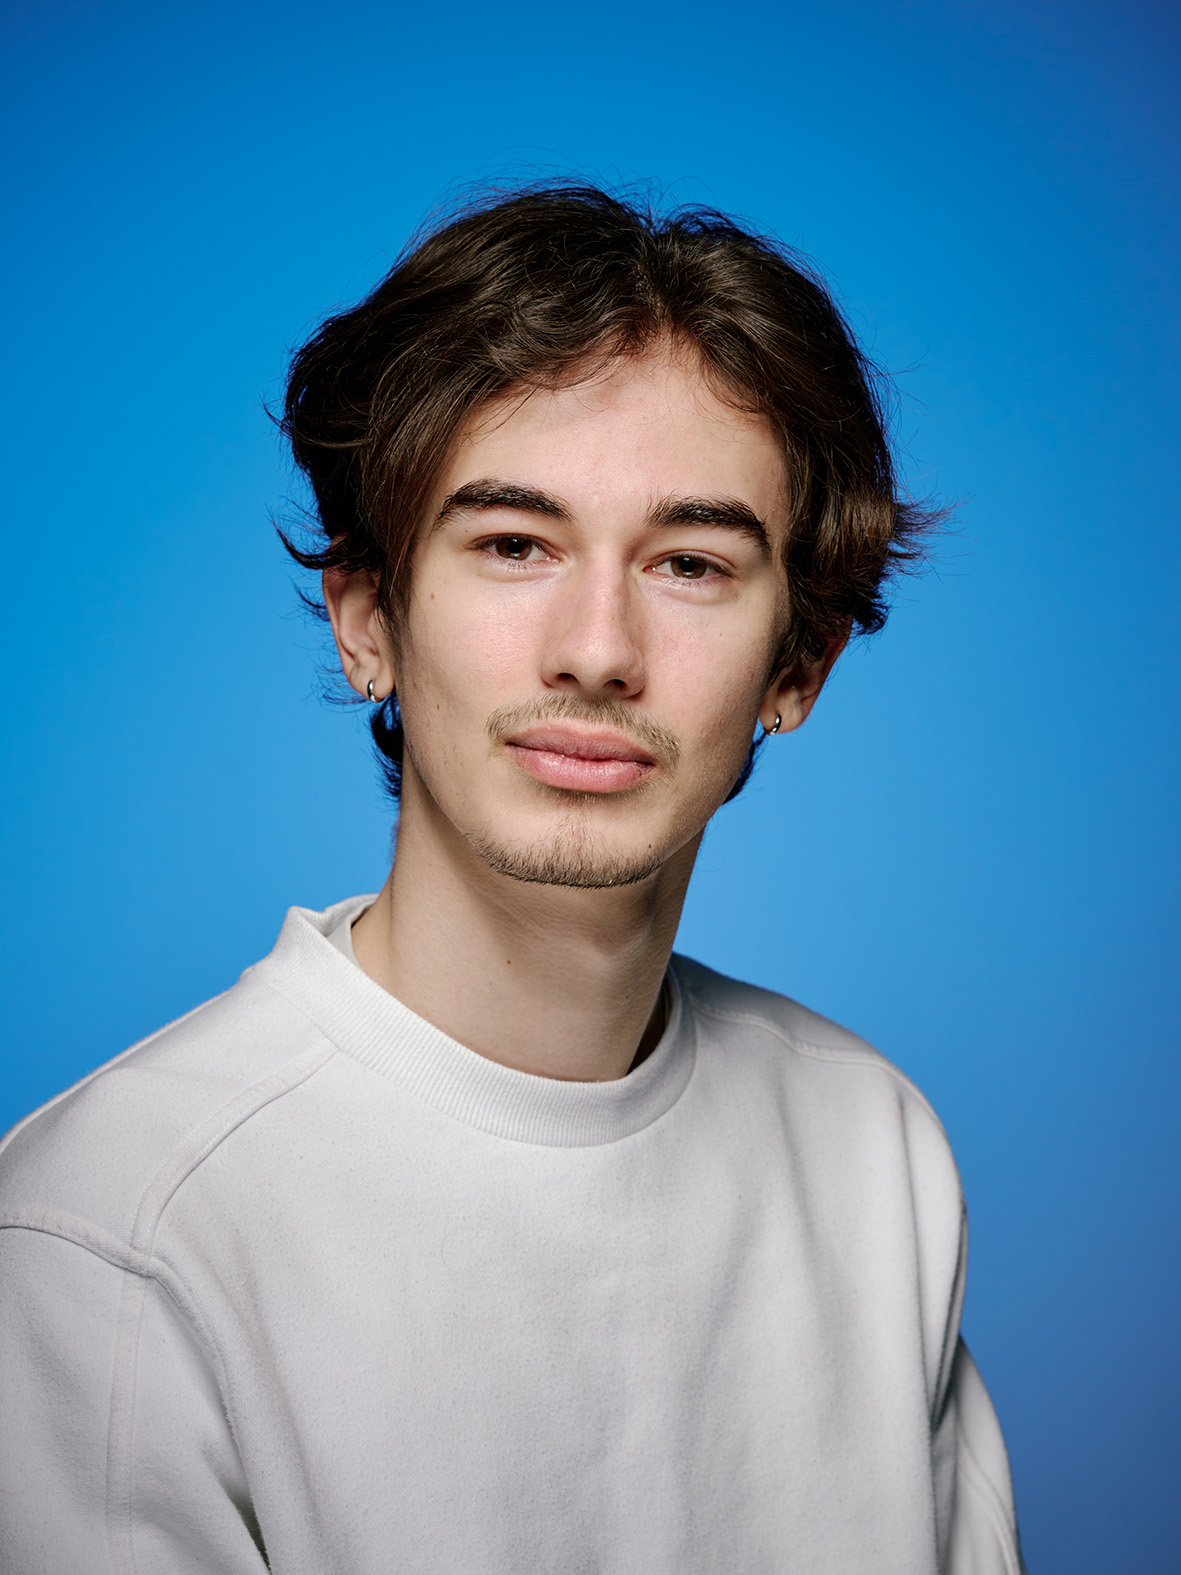
\includegraphics[width=80pt]{photo}
  }
  \hspace{1em}%
  \parbox[b]{0.7\textwidth}{
    {\Huge\bfseries\textcolor{blue!70!black}{Camille Maslin}}\\[0.2em]
    {\small \textcolor{gray}{Tours, France}}\\[0.5em]
    {\small
    \faMobile~+33 6 25 87 56 93 \quad
    \faEnvelope~\href{mailto:camillemaslin@gmail.com}{camillemaslin@gmail.com}\\[0.3em]
    \faLinkedin~\href{https://linkedin.com/in/camille-maslin}{camille-maslin} \quad
    \faGithub~\href{https://github.com/camille-maslin}{camille-maslin}\\[0.3em]
    \faGlobe~{\textbf{Portfolio :} \href{https://camille-maslin.github.io/Portfolio/}{\textcolor{blue}{camille-maslin.github.io/Portfolio}}}
    }
  }
  \vspace{1em}
  \hrule height 0.5pt \vspace{1em}
}

\begin{document}

\makecvtitle

% Objectifs
\section{Objectifs}
\cvitem{Court Terme}{Intégrer une école pour approfondir mes connaissances en développement et optimisation d'IA.}
\cvitem{Long Terme}{Contribuer à la recherche ou au développement d'innovations en intelligence artificielle.}

% Formation
\section{Formation}
\cventry{2025 (en cours)}{BUT Informatique, 3e année}{IUT de Dijon}{}{}{Parcours : Réalisation d'Applications, Conception, Développement et Validation.}
\cventry{2022}{Baccalauréat Scientifique}{Lycée Grandmont, Tours}{}{}{}

% Expérience Professionnelle en Informatique
\section{Expériences Professionnelles en Informatique}
\cventry{2025}{Stage de 3e année}{Laboratoire CIAD, Dijon}{16 semaines}{}{
\begin{itemize}
  \item Évaluation et implémentation de réseaux de neurones à impulsion (SNN).
  \item Développement en Python pour des cas d'usage complexes (gestes, labyrinthe, etc.).
\end{itemize}}
\cventry{2024}{Stage de 2e année}{Tours Métropole, Tours}{9 semaines}{}{
\begin{itemize}
  \item Migration et restructuration de bases de données PostgreSQL vers Oracle.
  \item Analyse des performances et recommandations d'optimisation.
\end{itemize}}

% Projets Personnels et Encadrés
\section{Projets Personnels et Encadrés}
\cvitem{\textbf{SecureCard-AI}}{
Développement d'un système de détection de fraude par carte bancaire utilisant le machine learning. Résultat : 99,97\% de précision sur plus de 57 000 transactions. {\textit{\textcolor{gray}{Projet personnel}}}}
\cvitem{\textbf{NeuroDraw-NN}}{
Implémentation from scratch d'un réseau de neurones pour la reconnaissance de chiffres en temps réel avec interface de dessin interactive. {\textit{\textcolor{gray}{Projet personnel}}}}
\cvitem{\textbf{Détection de Tumeurs}}{
Développement d'un modèle CNN en Python pour la classification d'IRM cérébrales. Résultat : 94\% de précision. {\textit{\textcolor{gray}{Projet personnel}}}}
\cvitem{\textbf{Visionneur d'Images}}{
Conception d'une application Python pour visualisation d'images multispectrales (laboratoire ImViA, Dijon). {\textit{\textcolor{gray}{Projet encadré}}}}
\cvitem{\textbf{Site Portfolio}}{
Création d'un site web responsive professionnel en HTML, CSS et JavaScript pour présenter efficacement mes réalisations. {\textit{\textcolor{gray}{Projet personnel}}}}

% Compétences
\section{Compétences}
\cvitem{Langages}{Python, C\#, C++, HTML/CSS, PHP.}
\cvitem{Bases de données}{SQL, Neo4j, Excel, Power BI.}
\cvitem{Outils}{Git, TensorFlow, Keras, OpenCV, VirtualBox.}
\cvitem{Savoir-être}{Communication, Autonomie, Adaptabilité.}
\cvitem{Langues}{\textbf{Anglais} : Niveau B2.}

% Centres d'Intérêt
\section{Centres d'Intérêt}
\cvitem{Passions}{Intelligence artificielle, science des données, guitare classique, escalade.}

\end{document}